\chapter{Implementação do Sistema} \label{cap:implementacao}
Este capítulo tem como propósito clarificar e justificar as várias decisões que tomámos no desenvolvimento dos vários módulos do projeto. Na secção \ref{mods} vamos apresentar uma visão geral dos componentes do projeto e as suas implementações, enquanto que nas secções seguintes vamos analisar esses componentes em mais detalhe, mais concretamente, na secção \ref{modww} vamos abordar o módulo WaterWatcher, na secção \ref{modwws} o módulo WaterWatcherService e na secção \ref{modsc} o módulo que simula o sistema da companhia fornecedora de água.\\

/* ---------------------NÃO ATUALIZADO
No ecrã de informações e estatísticas, a obtenção das contagens do cliente ocorre apenas no carregamento da página, sendo obtidas todas as contagens desse cliente, para todos os seus contadores e de todos os anos. Assim, quando o utilizador seleciona as contagens de um determinado ano e contador para serem apresentadas no gráfico, a aplicação apenas filtra as contagens já obtidas, de forma a reduzir os pedidos ao sistema da empresa, de forma a diminuir o tempo de apresentação dos resultados pela aplicação e para efetuar o número mínimo de pedidos possível a outros sistemas.
-----------------*/

\section{Módulos do Sistema} \label{mods} %Modulos------------------------------------------------------------
Este sistema, por ser desenvolvido na plataforma Outsystems, é constituído por módulos, que representam os vários elementos do sistema.\\
O módulo onde será desenvolvido o servidor e a interface para os utilizadores é o módulo WaterWatcher. O módulo que servirá para manter os dados será o WaterWatcherService.\\
Por fim desenvolvemos também um módulo de testes (WaterWatcherTests) e um módulo que simula as interações com o sistema informático da empresa fornecedora de água, denominado SimulCompany.

\section{Módulo WaterWatcher} \label{modww} %Water Watcher-----------------------------------------------
Este módulo é onde serão desenvolvidos a aplicação para os utilizadores e a lógica do servidor. Sendo assim, este módulo está dependente dos módulos WaterWatcherService e SimulCompany, sendo estas as únicas dependências entre os módulos do projeto.\\
Decidimos implementar a aplicação e o servidor no mesmo módulo dado que a plataforma nos permite implementar ações específicas do servidor ou do cliente num mesmo módulo, podendo distinguir quais os processos que irão ser executados nos servidores da aplicação ou no dispositivo dos clientes sem ser necessário criar mais estruturas de código.\\
Este módulo implementa toda a lógica e as vistas da aplicação para os utilizadores.

\section{Módulo WaterWatcherService} \label{modwws} %Water Watcher Service------------------------------
Este módulo é onde implementamos toda a lógica relativa ao armazenamento de informações que vamos utilizar neste sistema. No diagrama [ adicionar diagrama] podemos observar uma representação gráfica das várias entidades que armazenamos.\\
Os clientes têm os todos os atributos propostos na secção \ref{sec:dados} e têm ainda um atributo único que os identifica denominado idUser, que é gerado automaticamente aquando da criação de um novo utilizador. Este identificador é também o identificador de outra estrutura, que é a estrutura User. Esta estrutura contém as mesmas informações da estrutura Cliente, porém como esta é uma estrutura em qual a autenticação em aplicações construídas nesta plataforma se baseia \cite{outs:users} não poderíamos substituí-la.

\section{Módulo de Testes SimulCompany} \label{modsc}

\section{Registo no Sistema} \label{sec51}
O registo no sistema segue o processo representado na figura \ref{fig:registo}.

\begin{figure}[h!]
\begin{center}
\resizebox{120mm}{!}{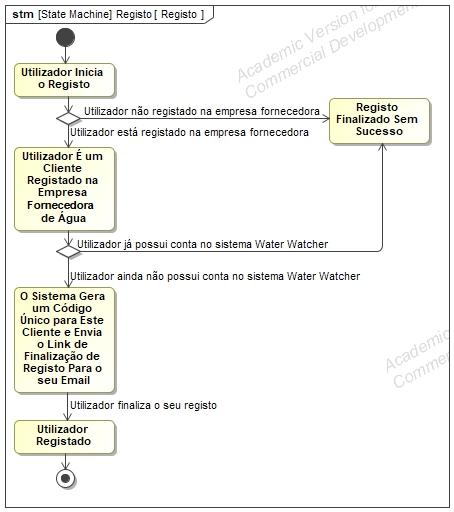
\includegraphics{diagramas/svg/Registo.jpg}}
\caption{Processo de registo no sistema.}
\label{fig:registo}
\end{center}
\end{figure}

Como descrito na figura, após o utilizador iniciar o registo e indicar o seu número de cliente, o sistema verifica se existe algum cliente registado na empresa fornecedora com esse número de cliente. Caso não exista nenhum cliente, é apresentada uma mensagem de erro. Se existir, o sistema verifica agora se este cliente já se encontra registado no serviço. Caso já se encontre registado, não será possível criar uma nova conta para este cliente, sendo assim apresentada uma nova mensagem de erro.\\
Sabendo agora que o cliente existe e não tem conta no sistema, é enviado um link para o email associado à conta do cliente no sistema da empresa fornecedora de água. Este link contém um código único gerado aleatoriamente que permitirá ao utilizador finalizar o seu registo, definindo uma palavra-passe. Após este registo, o sistema obtém as informações deste cliente na empresa fornecedora e é então gerado um novo utilizador no sistema .\\
Para a geração deste código único e aleatório, recorremos à biblioteca RNGCryptoServiceProvider \cite{RNGCryptoServiceProvider} onde geramos um código de 20 caracteres (letras maiúsculas, minúsculas e números). Ao início deste código vai ser adicionado o número de cliente seguido por um ‘.’ , para que possamos identificar o cliente ao qual o código está associado apenas pelo código em si. Este código é depois apagado do sistema após o registo do cliente.

\section{Captura de Imagem para Reconhecimento de Caracteres} \label{sec52}

Quando o utilizador inicia o processo de envio da fotografia do seu contador, a câmara do seu dispositivo é ativada e este é encaminhado para um ecrã onde que transmite o que a câmara está a captar, aparecendo no centro do ecrã uma moldura retangular azul. O utilizador deve alinhar os algarismos que mostram a leitura (com fundo preto) com a moldura, como representado na figura \ref{fig:moldura}, dado que o sistema vai apenas recolher a imagem que está contida nessa moldura.\\
Posteriormente, a aplicação móvel envia a imagem para o servidor, local onde será feito o OCR.

\begin{figure}[h!]
\begin{center}
\resizebox{120mm}{!}{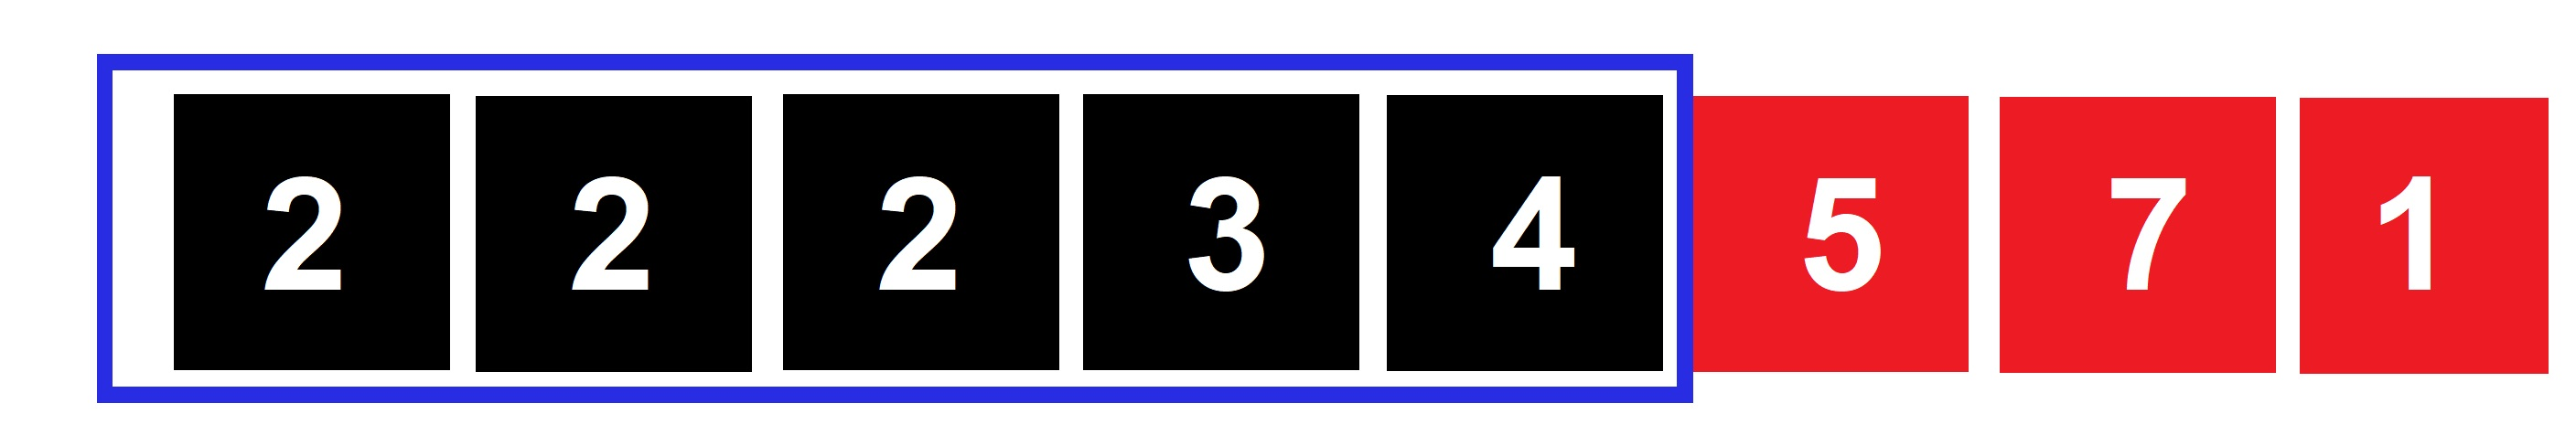
\includegraphics{diagramas/moldura.jpg}}
\caption{Esquematização do alinhamento da moldura com os caracteres da medição de água.}
\label{fig:moldura}
\end{center}
\end{figure}

\section{Reconhecimento de Caracteres} \label{sec53}

Para o reconhecimento de caracteres elaborámos uma extensão Outsystems que tem por base a biblioteca Tessreact \cite{tesseract}. O ficheiro de configuração utilizado foi o [testar os vários ficheiros digits]. 



















